\documentclass[11pt,a4paper]{article}
\usepackage[a4paper,margin=2.2cm]{geometry}
\usepackage[T1]{fontenc}\usepackage[utf8]{inputenc}
\usepackage{amsmath,booktabs,longtable,array,graphicx,float,hyperref,caption,subcaption}
\usepackage{microtype}\usepackage{parskip}
\hypersetup{hidelinks}\renewcommand{\thetable}{S\arabic{table}}\renewcommand{\thefigure}{S\arabic{figure}}
\begin{document}
\begin{center}{\Large\bfseries QMOF-Rec: Revised Supplementary Material}\\[5pt]
Authoritative final protocol and reviewer experiments, 19 September 2026\end{center}
\section*{Provenance and interpretation}
\label{sec:provenance}
The executable repository is \texttt{qmof-rec}, commit \texttt{10082124cf81a90ce40b4bd6306862416a46d2e6}. Source hashes, raw candidate pools, rankings, and reproduction comparisons accompany the artifacts. Twenty-one mask-aware regression tests pass. All seven primary methods reproduce Rel@5, NDCG@5, and diversity at the original four-decimal precision. There are five scenarios and ten seeds (42--51), not 50 independent scientific queries. Density is observed for 20,372 records, band gap for 10,810, and void fraction for none. Historical artifacts absent from this checkout are not asserted to have been reproduced.
\section*{Complete scenario-level ranking results}
\label{sec:scenario_results}
Metrics are computed on the same pool of 100 for each query/seed. Values below are means over ten seeds. MMR (top-5) exactly matches the original MMR top five in all 50 runs. DE uses the same representation and evaluation but a fixed list objective and 1,800 portfolio evaluations. Relevance/NDCG are aligned utility diagnostics, not independent labels.

\begin{footnotesize}\begin{longtable}{llrrrrr}
\caption{Complete primary-method results by scenario. SD describes diversity across seeds.}\label{tab:scenario}\\
\toprule
Scenario & Method & Rel@5 & NDCG & Diversity & SD & ms\\\midrule\endfirsthead
\toprule Scenario & Method & Rel@5 & NDCG & Diversity & SD & ms\\\midrule\endhead
CO$_2$ & WeightedSum & 0.7599 & 1.0000 & 0.0163 & 0.0000 & 0.05\\
CO$_2$ & LEA & 0.7599 & 1.0000 & 0.0288 & 0.0026 & 85.66\\
CO$_2$ & TOPSIS & 0.7599 & 1.0000 & 0.0163 & 0.0000 & 1.18\\
CO$_2$ & ParetoCrowding & 0.7599 & 1.0000 & 0.0297 & 0.0008 & 224.13\\
CO$_2$ & MMR (top-5) & 0.7599 & 1.0000 & 0.0333 & 0.0011 & 12.65\\
CO$_2$ & Random & 0.7377 & 0.9644 & 0.0189 & 0.0043 & 0.05\\
CO$_2$ & SemanticOnly & 0.7265 & 0.9395 & 0.0228 & 0.0035 & 0.04\\
CO$_2$ & DE portfolio & 0.7599 & 1.0000 & 0.0349 & 0.0014 & 70.24\\
Photocatalysis & WeightedSum & 0.8752 & 1.0000 & 0.0150 & 0.0000 & 0.05\\
Photocatalysis & LEA & 0.8752 & 1.0000 & 0.0150 & 0.0000 & 85.15\\
Photocatalysis & TOPSIS & 0.8752 & 1.0000 & 0.0150 & 0.0000 & 1.13\\
Photocatalysis & ParetoCrowding & 0.8752 & 1.0000 & 0.0150 & 0.0000 & 225.57\\
Photocatalysis & MMR (top-5) & 0.8752 & 1.0000 & 0.0150 & 0.0000 & 12.71\\
Photocatalysis & Random & 0.7624 & 0.8329 & 0.0232 & 0.0061 & 0.05\\
Photocatalysis & SemanticOnly & 0.7552 & 0.8245 & 0.0213 & 0.0049 & 0.04\\
Photocatalysis & DE portfolio & 0.8752 & 1.0000 & 0.0150 & 0.0000 & 70.36\\
Lightweight & WeightedSum & 0.9174 & 1.0000 & 0.0165 & 0.0000 & 0.05\\
Lightweight & LEA & 0.9174 & 1.0000 & 0.0193 & 0.0022 & 87.84\\
Lightweight & TOPSIS & 0.9174 & 1.0000 & 0.0165 & 0.0000 & 1.11\\
Lightweight & ParetoCrowding & 0.9013 & 0.9761 & 0.0378 & 0.0055 & 226.89\\
Lightweight & MMR (top-5) & 0.9174 & 1.0000 & 0.0204 & 0.0006 & 12.67\\
Lightweight & Random & 0.8967 & 0.9692 & 0.0266 & 0.0054 & 0.05\\
Lightweight & SemanticOnly & 0.8944 & 0.9665 & 0.0260 & 0.0032 & 0.04\\
Lightweight & DE portfolio & 0.9174 & 1.0000 & 0.0194 & 0.0011 & 68.89\\
Balanced & WeightedSum & 0.8979 & 1.0000 & 0.0165 & 0.0000 & 0.05\\
Balanced & LEA & 0.8979 & 1.0000 & 0.0194 & 0.0010 & 92.43\\
Balanced & TOPSIS & 0.8979 & 1.0000 & 0.0165 & 0.0000 & 1.13\\
Balanced & ParetoCrowding & 0.8979 & 1.0000 & 0.0185 & 0.0000 & 220.62\\
Balanced & MMR (top-5) & 0.8979 & 1.0000 & 0.0204 & 0.0006 & 12.73\\
Balanced & Random & 0.7647 & 0.8062 & 0.0256 & 0.0044 & 0.05\\
Balanced & SemanticOnly & 0.7548 & 0.7980 & 0.0250 & 0.0051 & 0.04\\
Balanced & DE portfolio & 0.8979 & 1.0000 & 0.0199 & 0.0012 & 68.92\\
Insulating & WeightedSum & 0.7893 & 1.0000 & 0.0293 & 0.0000 & 0.05\\
Insulating & LEA & 0.7893 & 1.0000 & 0.0294 & 0.0014 & 85.25\\
Insulating & TOPSIS & 0.7893 & 1.0000 & 0.0293 & 0.0000 & 1.08\\
Insulating & ParetoCrowding & 0.7893 & 1.0000 & 0.0303 & 0.0006 & 226.21\\
Insulating & MMR (top-5) & 0.7893 & 1.0000 & 0.0316 & 0.0018 & 12.77\\
Insulating & Random & 0.6860 & 0.8320 & 0.0241 & 0.0061 & 0.05\\
Insulating & SemanticOnly & 0.6693 & 0.8106 & 0.0249 & 0.0054 & 0.04\\
Insulating & DE portfolio & 0.7893 & 1.0000 & 0.0317 & 0.0011 & 68.51\\
\bottomrule\end{longtable}\end{footnotesize}
\section*{Joint gamma and redundancy sensitivity}
All 35 settings are rerun on all 50 pools. Changed sets and orders are counted relative to $(\gamma,\lambda)=(0.10,0.05)$. The true no-diversity ablation is $(0,0)$; setting only gamma to zero retains a diversity-dependent penalty. Full per-scenario, per-seed metrics and selected IDs are saved in \path{artifacts/reviewer_revision/sensitivity.csv}.

\begin{footnotesize}\begin{longtable}{rrrrrrr}
\caption{Joint sensitivity; identical rounded metrics can conceal different selected sets.}\\
\toprule
$\gamma$ & $\lambda$ & Rel@5 & NDCG & Diversity & Sets /50 & Orders /50\\\midrule\endfirsthead
\toprule $\gamma$ & $\lambda$ & Rel@5 & NDCG & Diversity & Sets /50 & Orders /50\\\midrule\endhead
0 & 0 & 0.8479 & 1.0000 & 0.0187 & 40 & 50\\
0 & 0.025 & 0.8479 & 1.0000 & 0.0224 & 0 & 0\\
0 & 0.05 & 0.8479 & 1.0000 & 0.0224 & 0 & 0\\
0 & 0.1 & 0.8479 & 1.0000 & 0.0224 & 0 & 0\\
0 & 0.2 & 0.8282 & 0.9707 & 0.0271 & 30 & 30\\
0.025 & 0 & 0.8479 & 1.0000 & 0.0215 & 39 & 50\\
0.025 & 0.025 & 0.8479 & 1.0000 & 0.0224 & 0 & 0\\
0.025 & 0.05 & 0.8479 & 1.0000 & 0.0224 & 0 & 0\\
0.025 & 0.1 & 0.8479 & 1.0000 & 0.0224 & 0 & 0\\
0.025 & 0.2 & 0.8282 & 0.9707 & 0.0271 & 30 & 30\\
0.05 & 0 & 0.8479 & 1.0000 & 0.0215 & 39 & 50\\
0.05 & 0.025 & 0.8479 & 1.0000 & 0.0224 & 0 & 0\\
0.05 & 0.05 & 0.8479 & 1.0000 & 0.0224 & 0 & 0\\
0.05 & 0.1 & 0.8479 & 1.0000 & 0.0224 & 0 & 0\\
0.05 & 0.2 & 0.8282 & 0.9707 & 0.0271 & 30 & 30\\
0.1 & 0 & 0.8479 & 1.0000 & 0.0215 & 39 & 50\\
0.1 & 0.025 & 0.8479 & 1.0000 & 0.0224 & 0 & 0\\
0.1 & 0.05 & 0.8479 & 1.0000 & 0.0224 & 0 & 0\\
0.1 & 0.1 & 0.8479 & 1.0000 & 0.0224 & 0 & 0\\
0.1 & 0.2 & 0.8282 & 0.9707 & 0.0271 & 30 & 30\\
0.2 & 0 & 0.8479 & 1.0000 & 0.0215 & 39 & 50\\
0.2 & 0.025 & 0.8479 & 1.0000 & 0.0224 & 0 & 0\\
0.2 & 0.05 & 0.8479 & 1.0000 & 0.0224 & 0 & 0\\
0.2 & 0.1 & 0.8479 & 1.0000 & 0.0224 & 0 & 0\\
0.2 & 0.2 & 0.8282 & 0.9707 & 0.0271 & 30 & 30\\
0.4 & 0 & 0.8479 & 1.0000 & 0.0215 & 39 & 50\\
0.4 & 0.025 & 0.8479 & 1.0000 & 0.0224 & 0 & 0\\
0.4 & 0.05 & 0.8479 & 1.0000 & 0.0224 & 0 & 0\\
0.4 & 0.1 & 0.8479 & 1.0000 & 0.0224 & 0 & 0\\
0.4 & 0.2 & 0.8282 & 0.9707 & 0.0271 & 30 & 30\\
0.8 & 0 & 0.8478 & 0.9999 & 0.0218 & 39 & 50\\
0.8 & 0.025 & 0.8478 & 0.9999 & 0.0219 & 13 & 35\\
0.8 & 0.05 & 0.8478 & 0.9999 & 0.0225 & 1 & 1\\
0.8 & 0.1 & 0.8477 & 0.9998 & 0.0226 & 1 & 1\\
0.8 & 0.2 & 0.8278 & 0.9703 & 0.0274 & 32 & 32\\
\bottomrule\end{longtable}\end{footnotesize}
\section*{Runtime dispersion and scaling}
Reranking times are serial wall-clock measurements; they exclude shared catalog scoring, retrieval, networking, and explanations. Table S3 summarizes 50 query/seed runs. The original MMR full-list row is an audit comparator, not the matched top-five implementation. Scaling uses 45 measurements per method/size (five queries, three seeds, three repeats), with population 30 and 60 LEA iterations fixed.

\begin{table}[H]\centering\small
\caption{Primary-method runtime dispersion; MMR without the top-5 suffix computes the full 100 ranks.}
\begin{tabular}{lrrrr}
\toprule
Method & Mean ms & SD ms & Minimum & Maximum\\\midrule
WeightedSum & 0.051 & 0.005 & 0.044 & 0.068\\
LEA & 87.264 & 10.326 & 81.479 & 153.210\\
TOPSIS & 1.125 & 0.111 & 0.993 & 1.567\\
ParetoCrowding & 224.682 & 11.216 & 207.015 & 291.763\\
MMR (top-5) & 12.704 & 0.275 & 12.109 & 13.462\\
Random & 0.051 & 0.004 & 0.045 & 0.065\\
SemanticOnly & 0.039 & 0.009 & 0.030 & 0.071\\
DE portfolio & 69.386 & 2.253 & 67.609 & 79.996\\
MMR & 2209.671 & 108.106 & 2068.668 & 2597.575\\
\bottomrule\end{tabular}\end{table}

\begin{footnotesize}\begin{longtable}{rlrrr}
\caption{Post-retrieval scalability at fixed top-five output.}\\
\toprule
Pool size & Method & Measurements & Mean ms & SD ms\\\midrule\endfirsthead
\toprule Pool size & Method & Measurements & Mean ms & SD ms\\\midrule\endhead
50 & WeightedSum & 45 & 0.029 & 0.015\\
50 & TOPSIS & 45 & 0.501 & 0.055\\
50 & LEA & 45 & 76.514 & 2.868\\
50 & MMR (top-5) & 45 & 6.056 & 0.137\\
100 & WeightedSum & 45 & 0.057 & 0.025\\
100 & TOPSIS & 45 & 1.000 & 0.103\\
100 & LEA & 45 & 82.996 & 0.604\\
100 & MMR (top-5) & 45 & 12.611 & 0.298\\
200 & WeightedSum & 45 & 0.120 & 0.047\\
200 & TOPSIS & 45 & 2.010 & 0.167\\
200 & LEA & 45 & 97.948 & 1.403\\
200 & MMR (top-5) & 45 & 25.611 & 0.402\\
500 & WeightedSum & 45 & 0.315 & 0.102\\
500 & TOPSIS & 45 & 4.990 & 0.318\\
500 & LEA & 45 & 140.972 & 7.039\\
500 & MMR (top-5) & 45 & 65.155 & 0.847\\
1000 & WeightedSum & 45 & 0.679 & 0.184\\
1000 & TOPSIS & 45 & 10.189 & 0.542\\
1000 & LEA & 45 & 229.754 & 76.462\\
1000 & MMR (top-5) & 45 & 137.550 & 30.063\\
\bottomrule\end{longtable}\end{footnotesize}
\section*{Descriptor-level screening sanity check}
Density is in g/cm$^3$ and band gap in eV. Means average the selected observed descriptors within each seed, then average across seeds with defined means; all-missing seed means are excluded, not zero-filled. A dash denotes an undefined summary. Catalog and pool are reference populations, not experimental control groups. Values are not adsorption capacity or evidence of synthesis feasibility. Missingness is reported separately; thresholds are descriptive. Formula and text heuristics can dominate the retained scenario definitions.

\begin{footnotesize}\begin{longtable}{llrrrr}
\caption{Observed descriptor means and band-gap completeness; the threshold percentage uses observed gaps as denominator.}\\
\toprule
Scenario & Group & Density & Gap & Gap missing \% & Gap $\geq$3.5 \%\\\midrule\endfirsthead
\toprule Scenario & Group & Density & Gap & Gap missing \% & Gap $\geq$3.5 \%\\\midrule\endhead
CO$_2$ & catalog & 1.696 & 3.858 & 46.9 & 64.5\\
CO$_2$ & candidate pool & 1.619 & 3.325 & 0.0 & 33.0\\
CO$_2$ & Random & 1.639 & 3.213 & 0.0 & 24.0\\
CO$_2$ & WeightedSum & 1.537 & 3.070 & 0.0 & 0.0\\
CO$_2$ & LEA & 1.640 & 2.116 & 0.0 & 0.0\\
Photocatalysis & catalog & 1.696 & 3.858 & 46.9 & 64.5\\
Photocatalysis & candidate pool & 1.647 & 2.922 & 0.0 & 0.0\\
Photocatalysis & Random & 1.662 & 2.912 & 0.0 & 0.0\\
Photocatalysis & WeightedSum & 0.870 & 2.804 & 0.0 & 0.0\\
Photocatalysis & LEA & 0.870 & 2.804 & 0.0 & 0.0\\
Lightweight & catalog & 1.696 & 3.858 & 46.9 & 64.5\\
Lightweight & candidate pool & 0.688 & 2.873 & 93.0 & 0.0\\
Lightweight & Random & 0.683 & 2.758 & 90.0 & 0.0\\
Lightweight & WeightedSum & 0.859 & 2.693 & 0.0 & 0.0\\
Lightweight & LEA & 0.890 & 2.911 & 0.0 & 0.0\\
Balanced & catalog & 1.696 & 3.858 & 46.9 & 64.5\\
Balanced & candidate pool & 1.518 & 3.021 & 0.0 & 12.0\\
Balanced & Random & 1.609 & 2.947 & 0.0 & 4.0\\
Balanced & WeightedSum & 0.859 & 2.693 & 0.0 & 0.0\\
Balanced & LEA & 0.871 & 2.801 & 0.0 & 0.0\\
Insulating & catalog & 1.696 & 3.858 & 46.9 & 64.5\\
Insulating & candidate pool & 1.594 & 4.307 & 0.0 & 100.0\\
Insulating & Random & 1.537 & 4.071 & 0.0 & 100.0\\
Insulating & WeightedSum & 0.771 & 4.211 & 0.0 & 100.0\\
Insulating & LEA & 0.810 & 4.311 & 0.0 & 100.0\\
\bottomrule\end{longtable}\end{footnotesize}
\section*{Ablation scope and advanced optimizer}
Zero-imputed WeightedSum changes the missing-score convention on the same pools, with evaluation using the original masked relevance. If its top five are unchanged, that is a null effect in this pool, not a demonstration that masking is unnecessary. Uniform-pool LEA replaces candidate generation with random sampling from the catalog and therefore changes the feasible set and NDCG ideal. Its scores cannot be read as a same-pool optimizer comparison. Proxy S/A variants use 85\% relevance and 15\% engineered proxy, not trained GNN output.

The DE portfolio implementation uses SciPy 1.13.1, \texttt{best1bin}, differential weight dithering 0.5--1, crossover 0.7, immediate updating, no polishing, 30 members, and 59 generations after initialization. Random keys select exactly five unique IDs. One population member encodes WeightedSum, with 29 random members. Its fixed list objective is $\overline R+0.1\overline B+0.1D-0.05e^{-D}$. Cached pairwise distance construction is included in timing; outputs are ordered by relevance. Tests verify scalar/vectorized masked-distance agreement, unique outputs, 1,800 evaluations, and utility no worse than the initial WeightedSum portfolio. Equal nominal search budgets do not equate candidate-fitness evaluations with whole-portfolio evaluations, nor establish identical optimization problems.

\section*{Implementation consistency and missingness}
The final protocol and configuration metadata specify eight formula coordinates, including heteroatom fraction. The executed hybrid vector contains two physical, eight formula, and two proxy dimensions, with block scaling $\sqrt{0.55/2}$, $\sqrt{0.30/8}$, and $\sqrt{0.15/2}$ before masked RMS distance. The missing physical gap coordinate is excluded, but proxy A has an internal zero fallback. This retained heuristic is disclosed rather than silently changed during reproduction. Objective remapping and hybrid diversity remain distinct. LEA retains best-ever candidate fitness across changing selected contexts; its trace is not convergence of a single fixed portfolio objective.

\section*{Explanation audit}
The runner emits 30 templates from saved seed-42 LEA selections. Groundedness uses identifier presence and limitation awareness uses phrases. Metadata consistency, nominal explanation-quality scores, and violation flags are assigned, rather than assessed by an independent evaluator. The former 5/5 and zero-hallucination claims are therefore excluded as evidence of explanation quality. No live LLM or expert-human benchmark has been run.

\section*{Reproduction commands and files}
Run from the authoritative repository:
\begin{verbatim}
PYTHONPATH=backend python3 -m pytest -q backend/tests
python3 scripts/run_final_diversity_aware_masked_protocol.py
python3 scripts/run_reviewer_revision.py
python3 scripts/build_reviewer_revision.py
\end{verbatim}
The baseline configuration is \path{configs/final_diversity_aware_masked_protocol.json}. New raw results, manifests, figures, and source snapshots are in \path{artifacts/reviewer_revision/}. The manuscript builder writes only the designated revision workspace and retains input sources under the executable repository's source snapshots. The versioned reproducibility archive \path{qmof-rec-v1.1-COMMT-revision.tar.gz} contains the frozen evidence, executable ranking code, regression tests, and a SHA-256 manifest.
\clearpage\section*{Historical interface illustrations}
The following screenshots are retained as interface illustrations. They are not new experiments, physical validation, or an independently assessed LLM benchmark.
\section*{CO$_2$ Adsorption Scenario}

\begin{figure}[H]
  \centering
  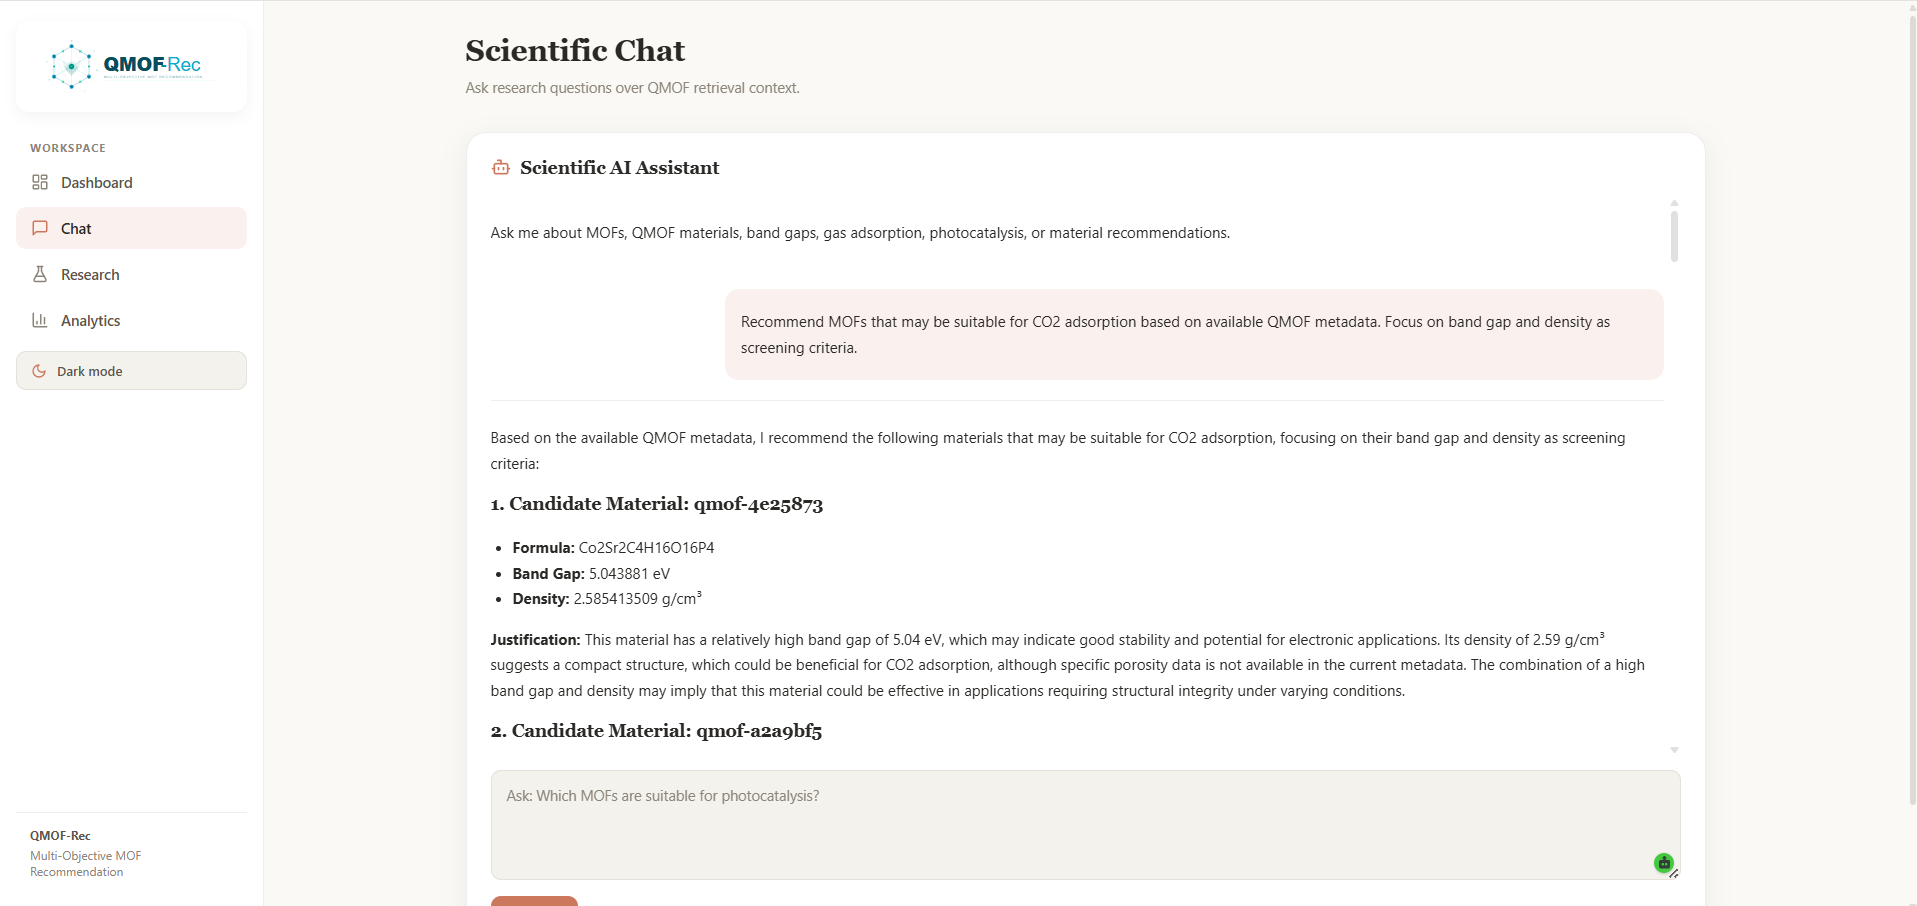
\includegraphics[width=\linewidth]{figures/Scenarion_1a-CO2.png}
  \caption{CO$_2$ adsorption scenario. The assistant recommends candidates based on available metadata and states that porosity and CO$_2$ uptake data are unavailable. Void fraction and adsorption uptake are unavailable in the current metadata.}
\end{figure}

\begin{figure}[H]
  \centering
  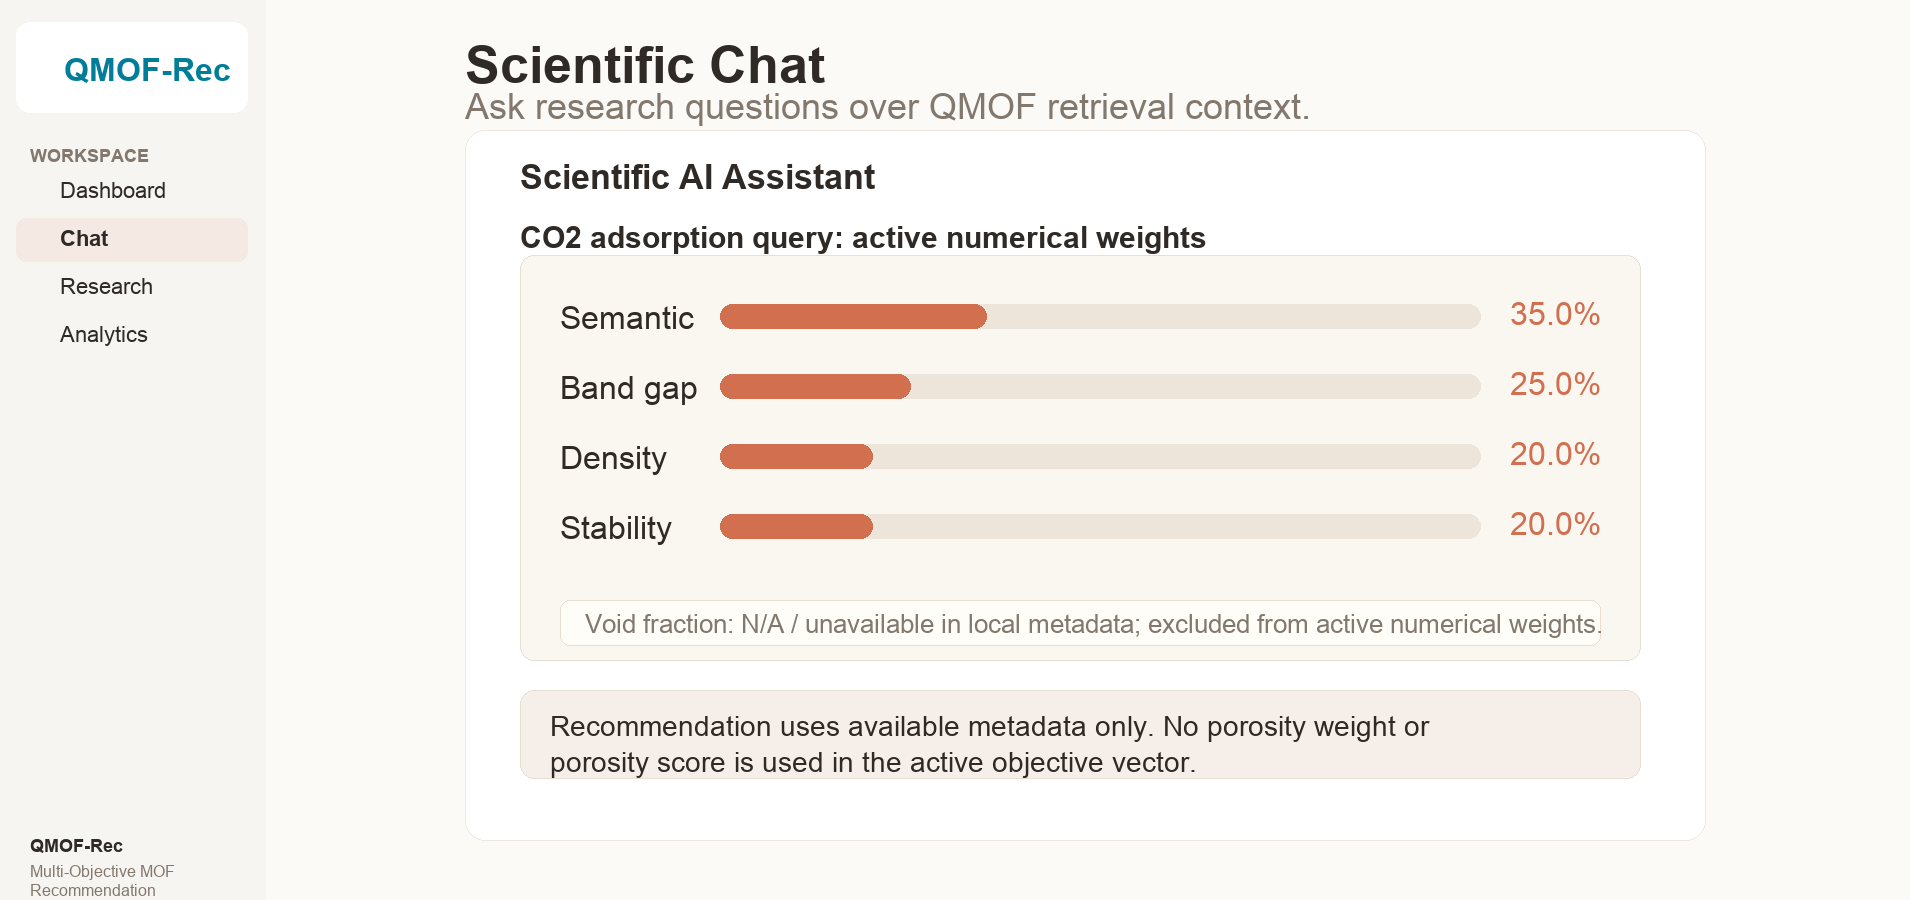
\includegraphics[width=\linewidth]{figures/Scenarion_1b-CO2.png}
  \caption{CO$_2$ adsorption scenario showing active numerical weights after excluding unavailable void-fraction information. Void fraction is displayed only as unavailable metadata and is not used as an active numerical objective, weight, or score.}
\end{figure}

\begin{figure}[H]
  \centering
  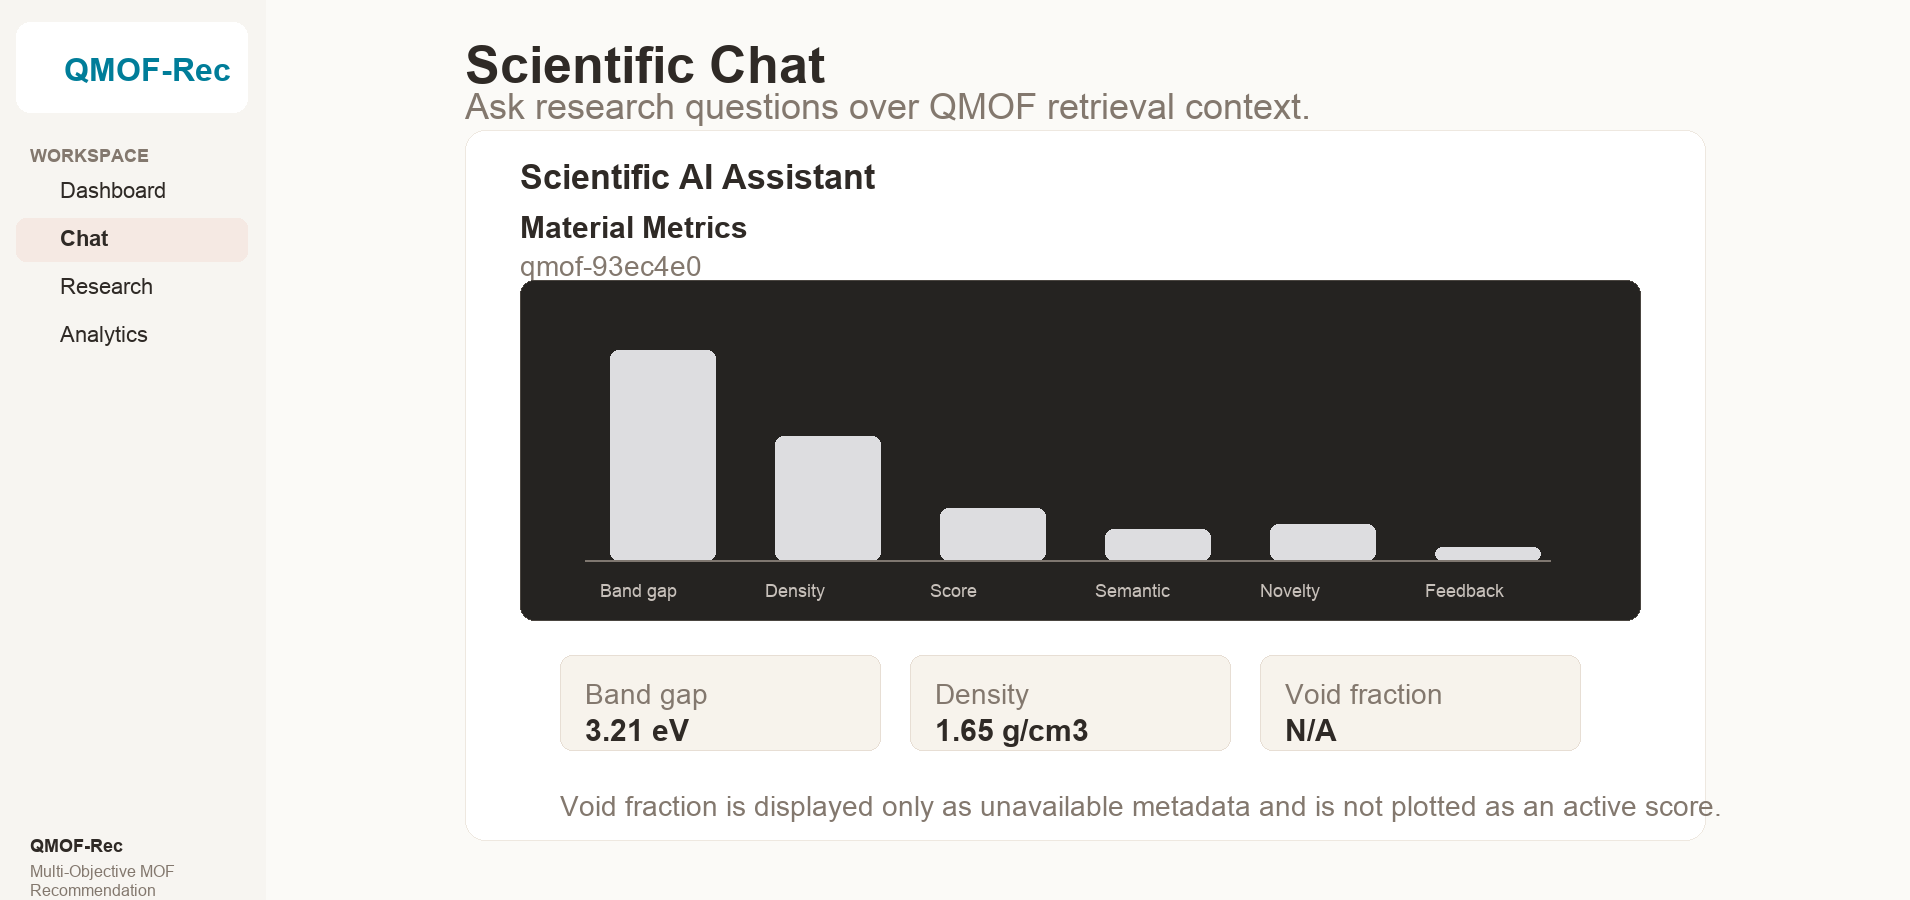
\includegraphics[width=\linewidth]{figures/Scenarion_1c-CO2.png}
  \caption{CO$_2$ adsorption scenario showing material metrics for a candidate record. In the revised implementation, void fraction is displayed only as unavailable metadata and is excluded from active numerical ranking.}
\end{figure}

\begin{figure}[H]
  \centering
  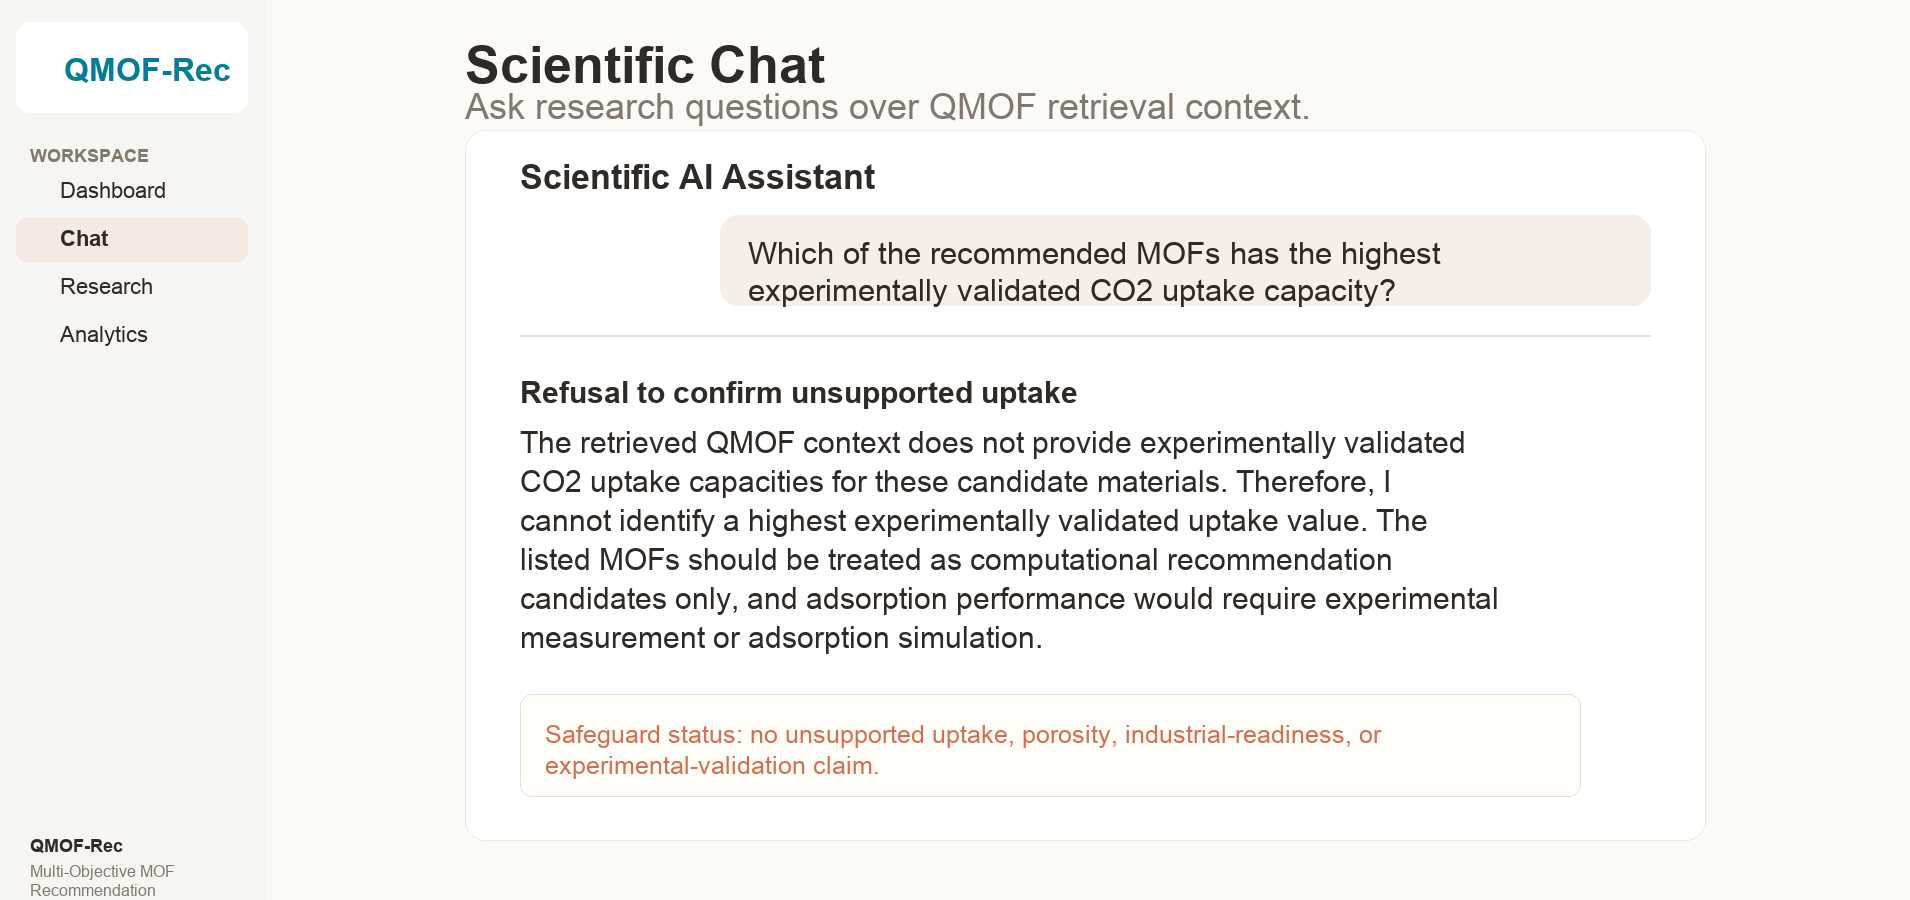
\includegraphics[width=\linewidth]{figures/Scenarion_1d-CO2.png}
  \caption{CO$_2$ adsorption scenario testing unsupported uptake claims. The assistant declines to identify experimentally validated CO$_2$ uptake because the retrieved context contains no experimentally validated uptake data.}
\end{figure}

\begin{figure}[H]
  \centering
  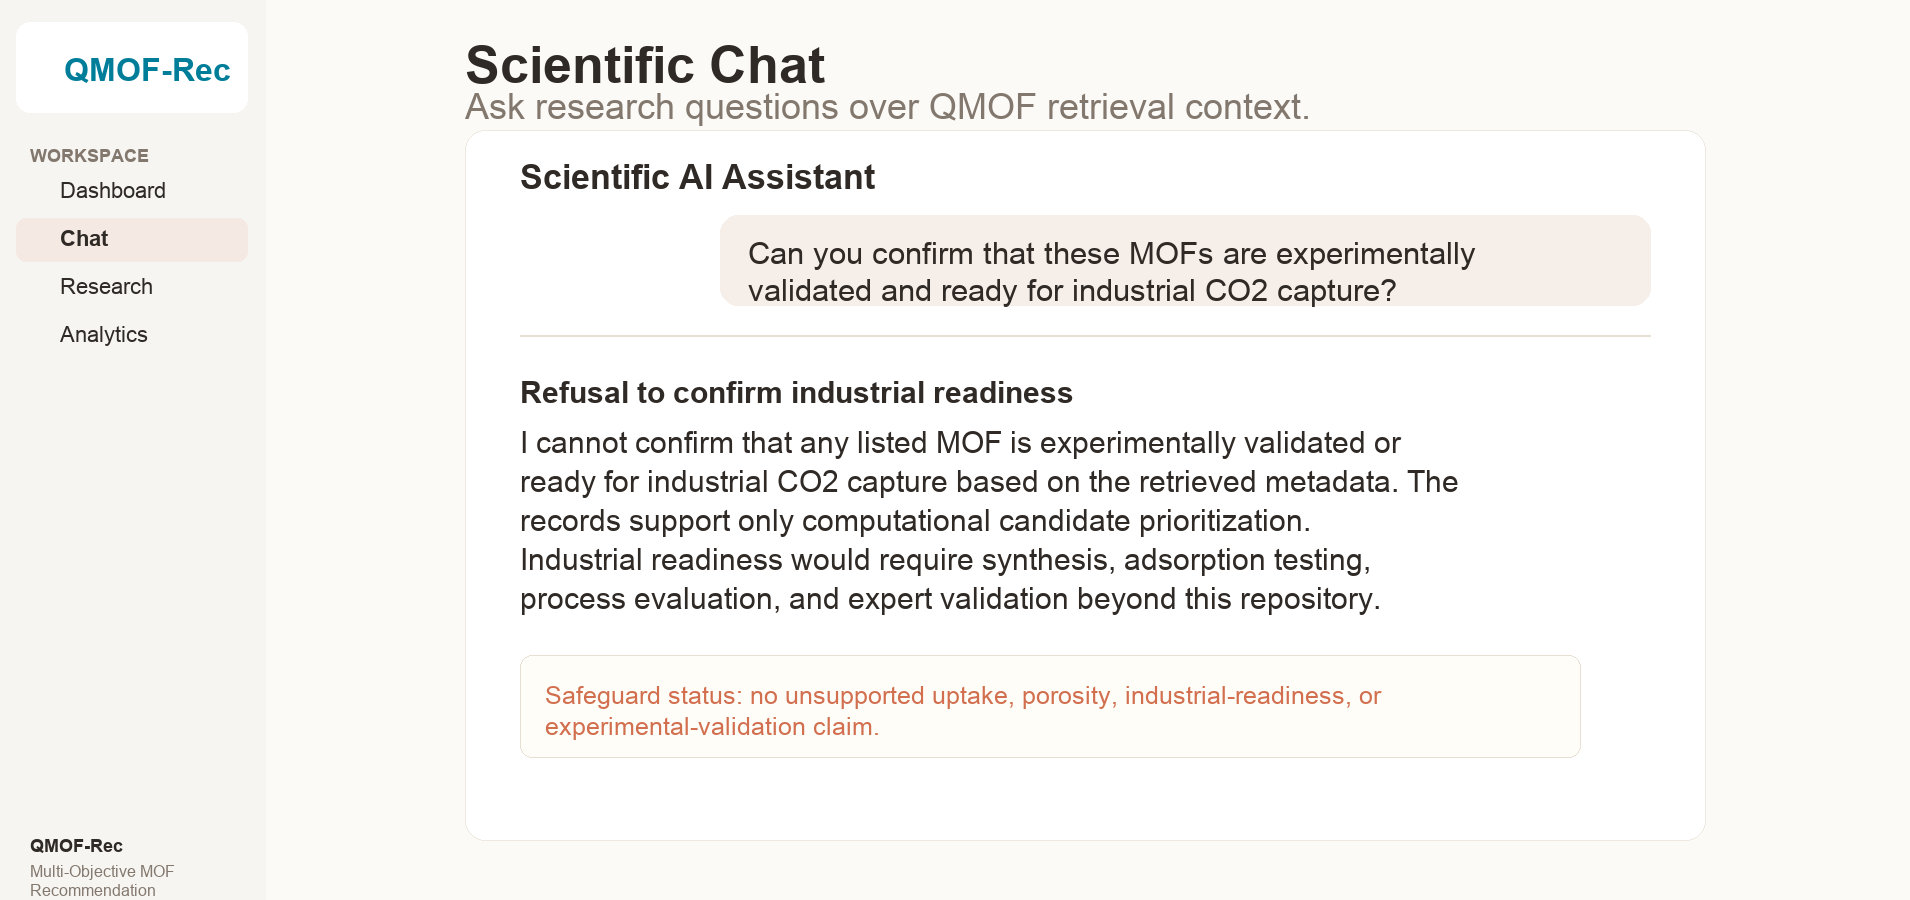
\includegraphics[width=\linewidth]{figures/Scenarion_1e-CO2.png}
  \caption{CO$_2$ adsorption scenario testing industrial-readiness claims. The assistant treats the listed MOFs as recommendation candidates requiring expert follow-up, not as experimentally validated capture materials.}
\end{figure}

\section*{Photocatalysis Scenario}

\begin{figure}[H]
  \centering
  \begin{subfigure}[b]{0.49\linewidth}
    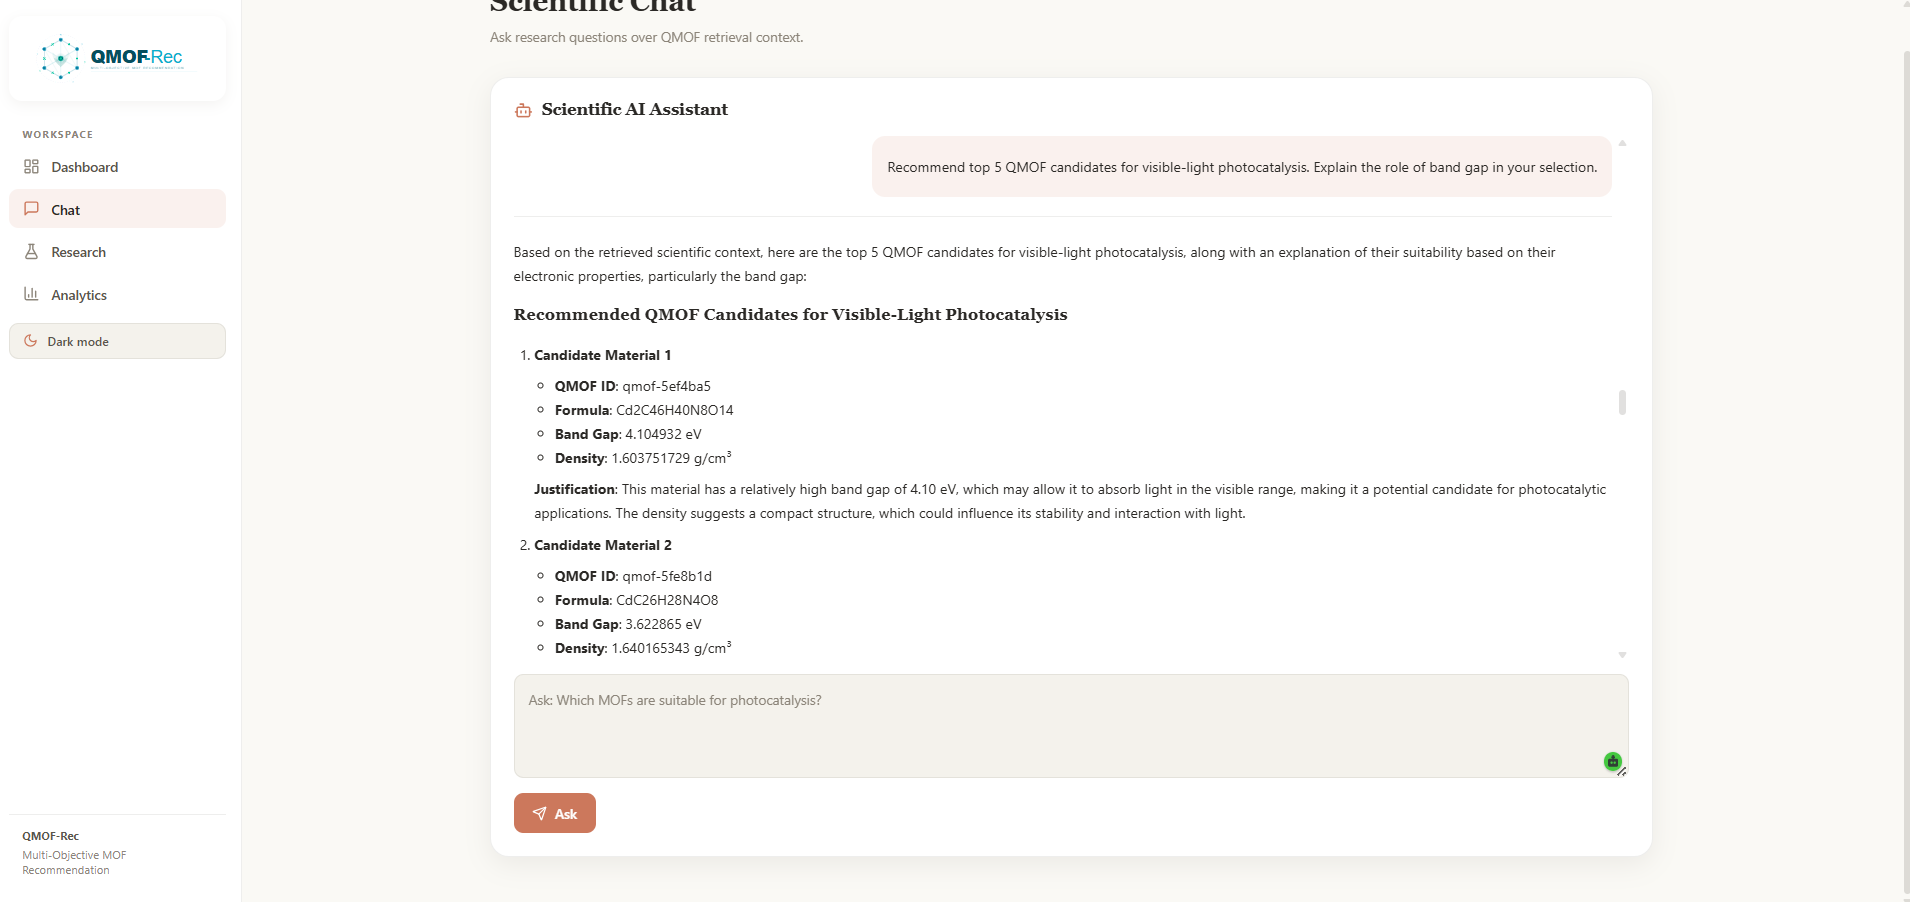
\includegraphics[width=\linewidth]{figures/Scenarion_2a-Photolytic.png}
    \caption{Top-5 photocatalysis candidates with band-gap-oriented justifications.}
  \end{subfigure}\hfill
  \begin{subfigure}[b]{0.49\linewidth}
    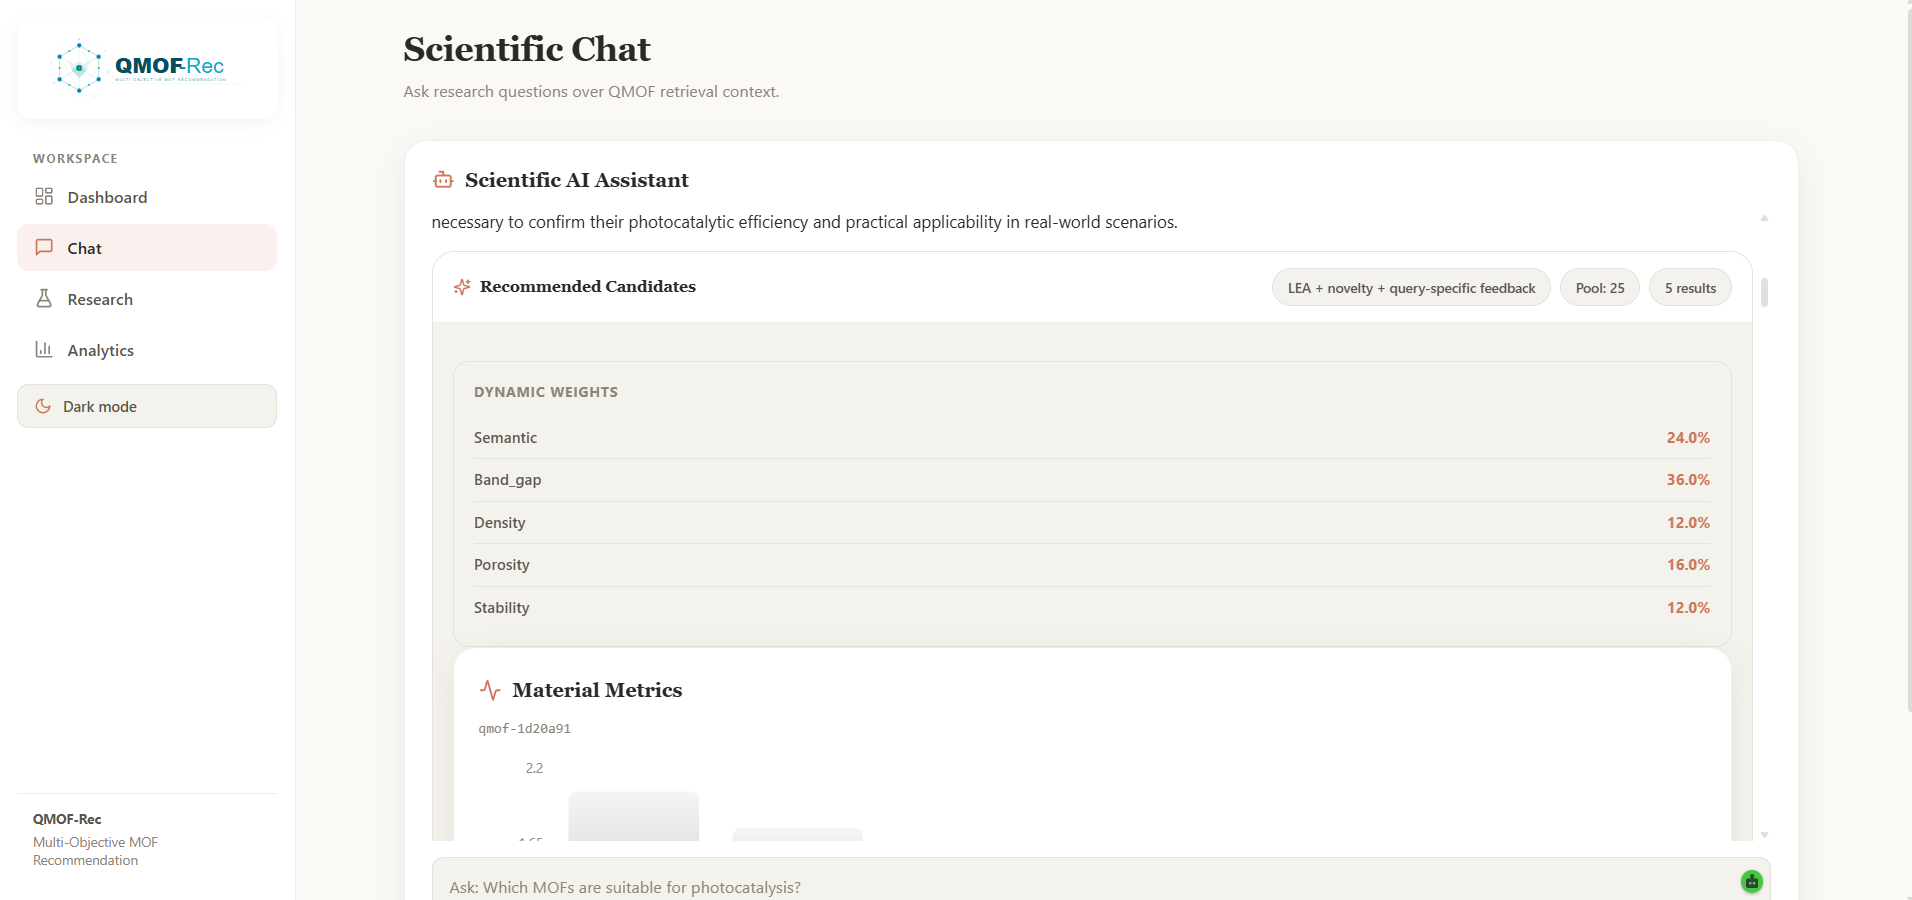
\includegraphics[width=\linewidth]{figures/Scenarion_2b-Photolytic.png}
    \caption{Dynamic objective weights for a photocatalysis-oriented query.}
  \end{subfigure}
  \caption{Photocatalysis scenario screenshots. These illustrate answer structure and interface behavior rather than physical validation.}
\end{figure}

\section*{Missing-Information Trap}

\begin{figure}[H]
  \centering
  \begin{subfigure}[b]{0.49\linewidth}
    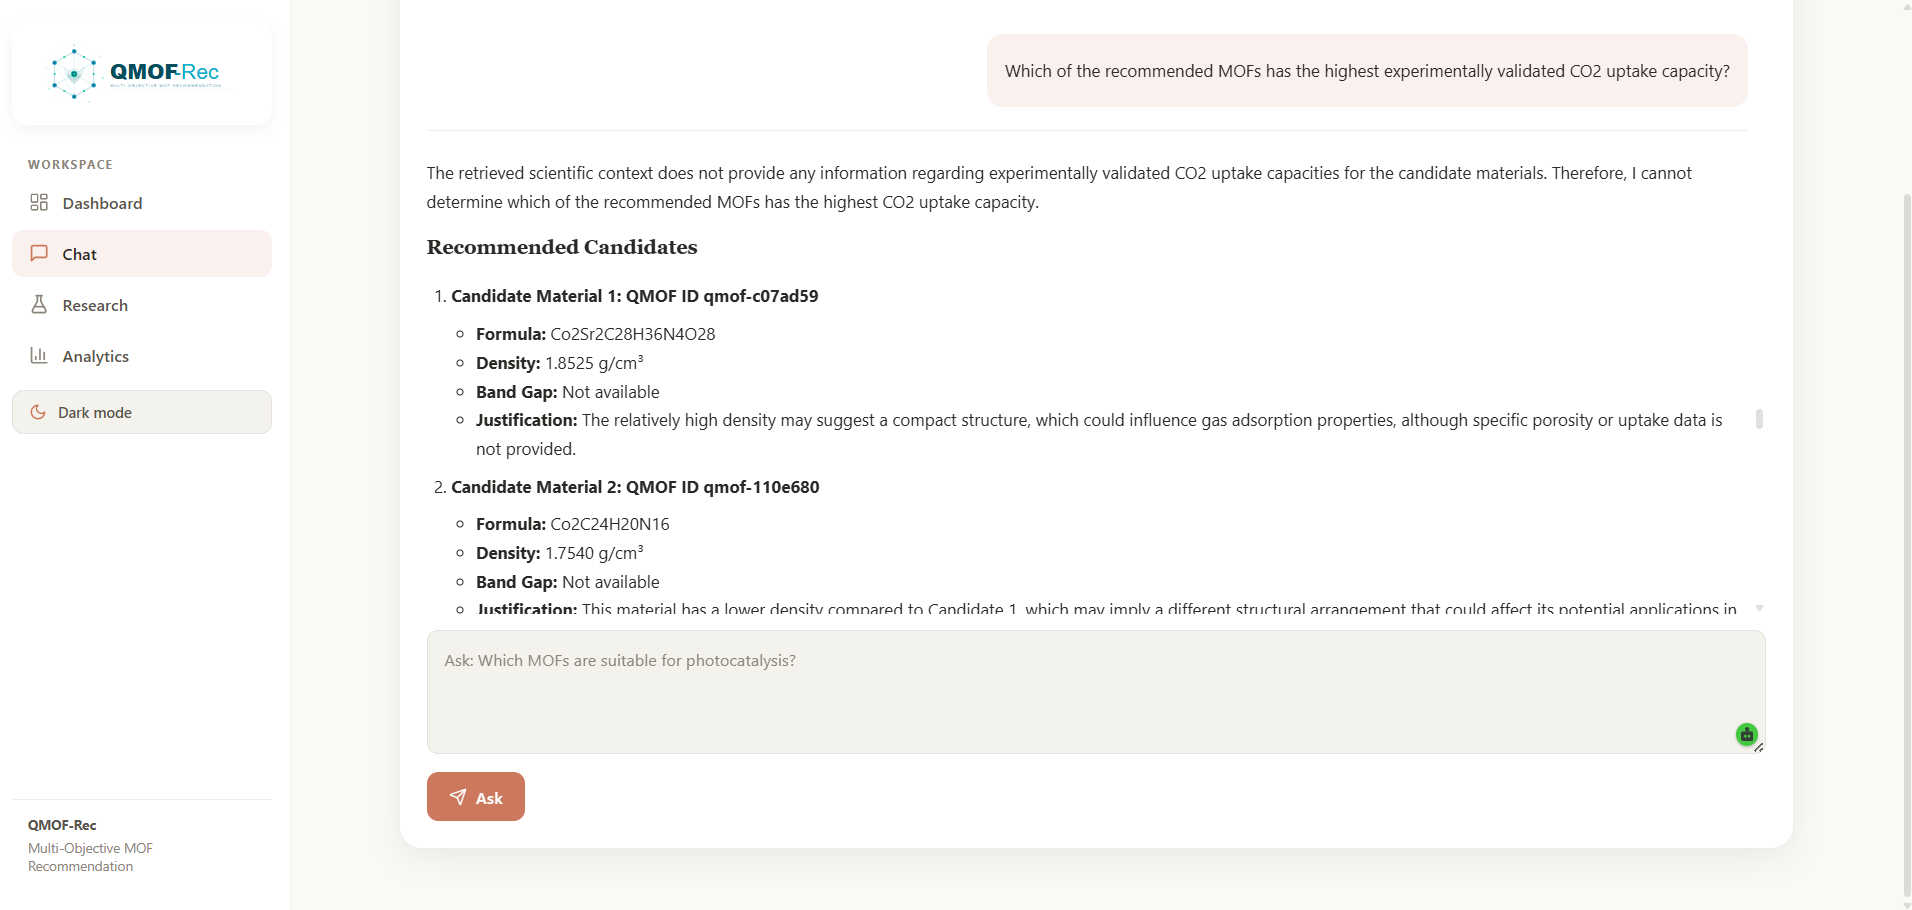
\includegraphics[width=\linewidth]{figures/Scenarion_3a-Hallusination.png}
    \caption{Refusal to confirm experimentally validated CO$_2$ uptake.}
  \end{subfigure}\hfill
  \begin{subfigure}[b]{0.49\linewidth}
    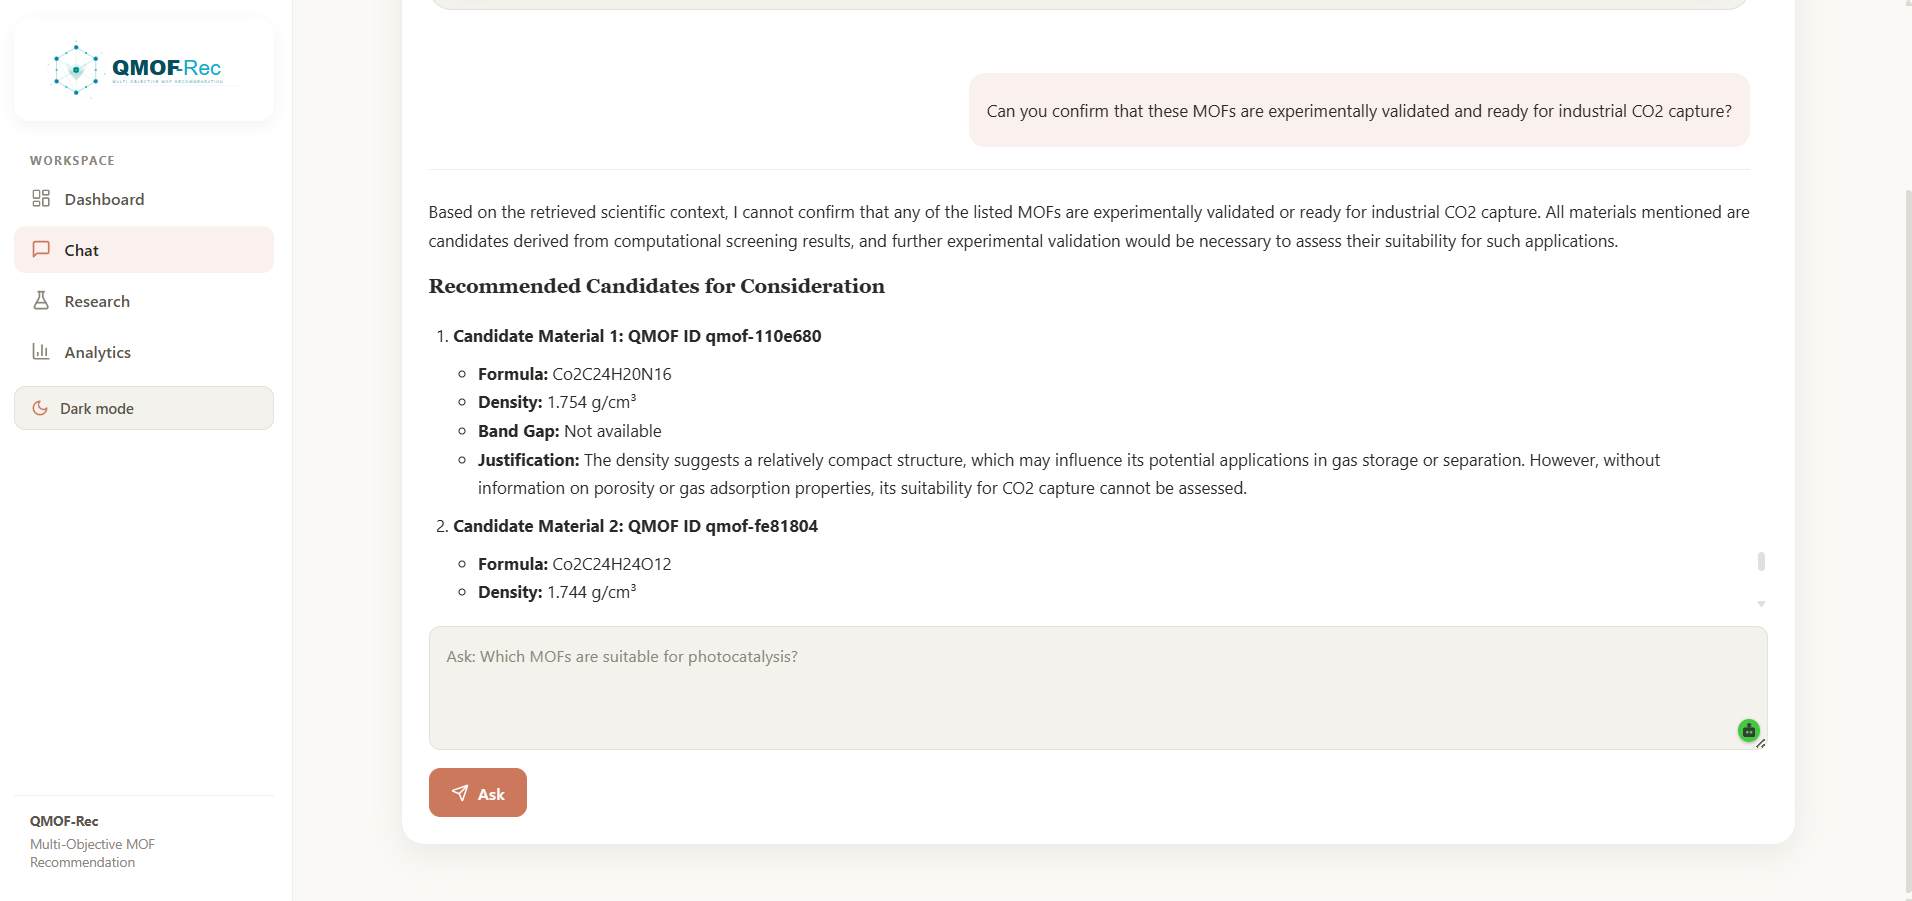
\includegraphics[width=\linewidth]{figures/Scenarion_3b-Hallusination.png}
    \caption{Refusal to confirm industrial readiness.}
  \end{subfigure}
  \caption{Missing-information trap screenshots. The assistant declines to fabricate experimental validation claims.}
\end{figure}

\section*{Lightweight Gas Storage}

\begin{figure}[H]
  \centering
  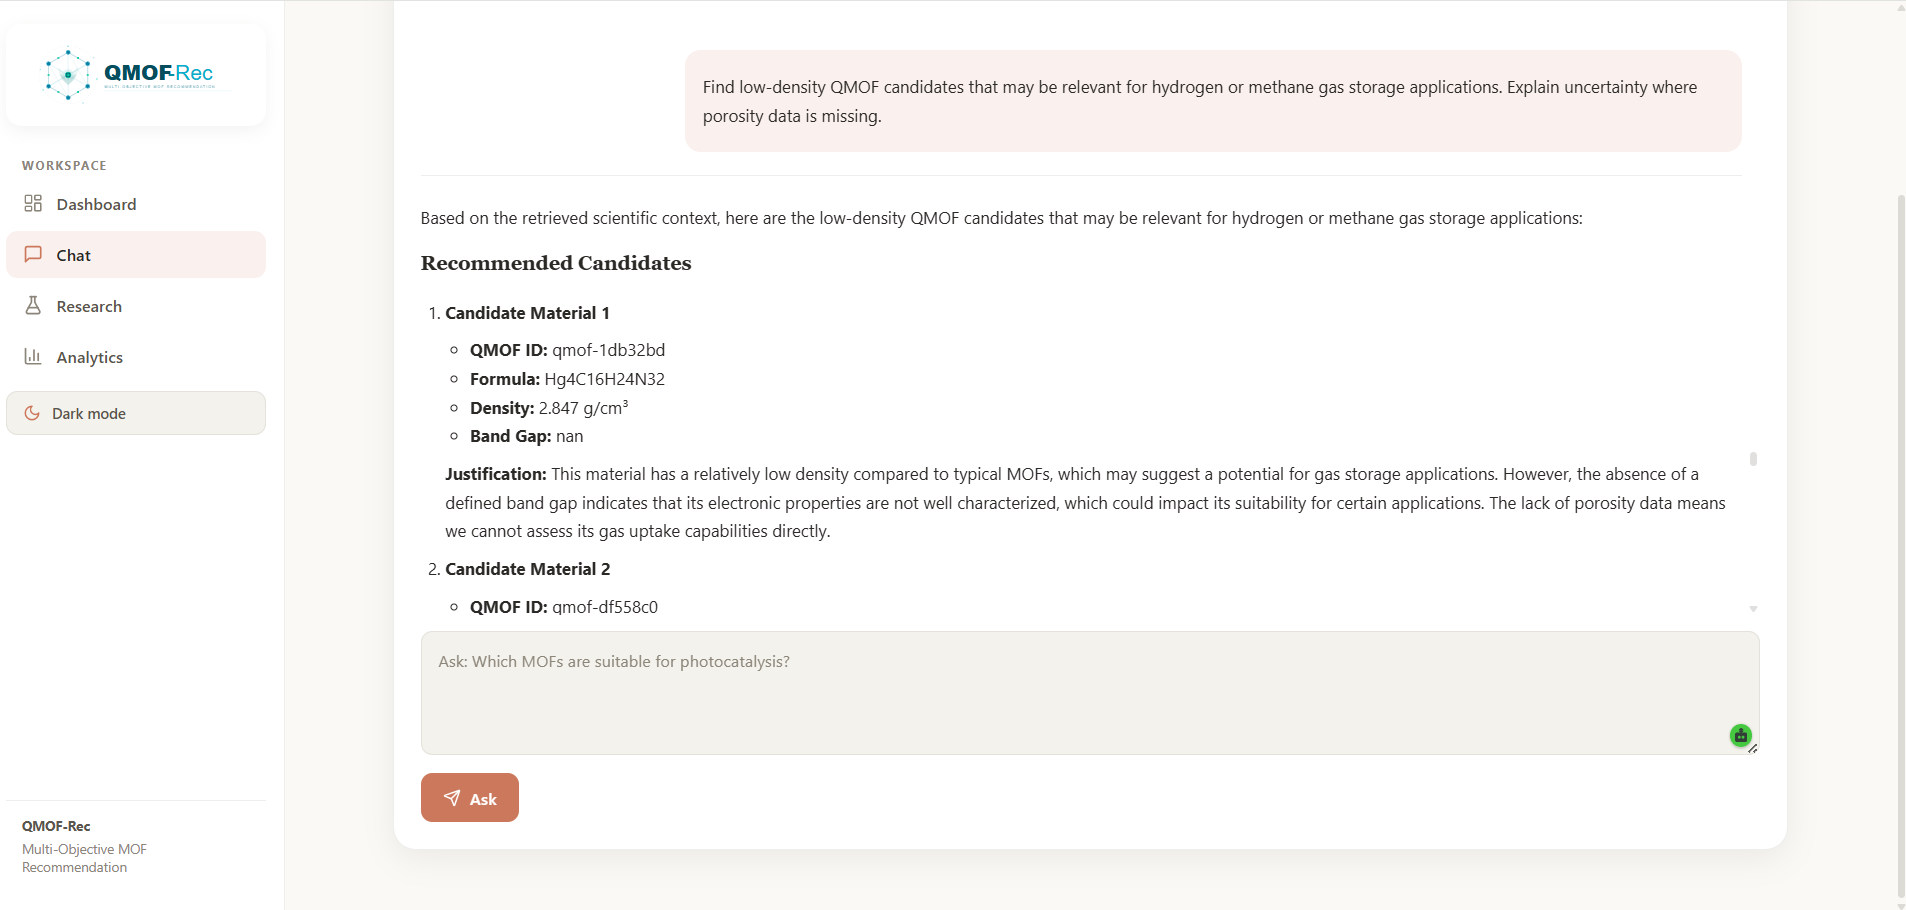
\includegraphics[width=\linewidth]{figures/Scenarion_4a-GasStorage.png}
  \caption{Lightweight gas-storage scenario. Candidate recommendations are based on available metadata such as density; void fraction, porosity, and gas uptake data are unavailable, so conclusions are preliminary.}
\end{figure}

\section*{Ranking Logic}

\begin{figure}[H]
  \centering
  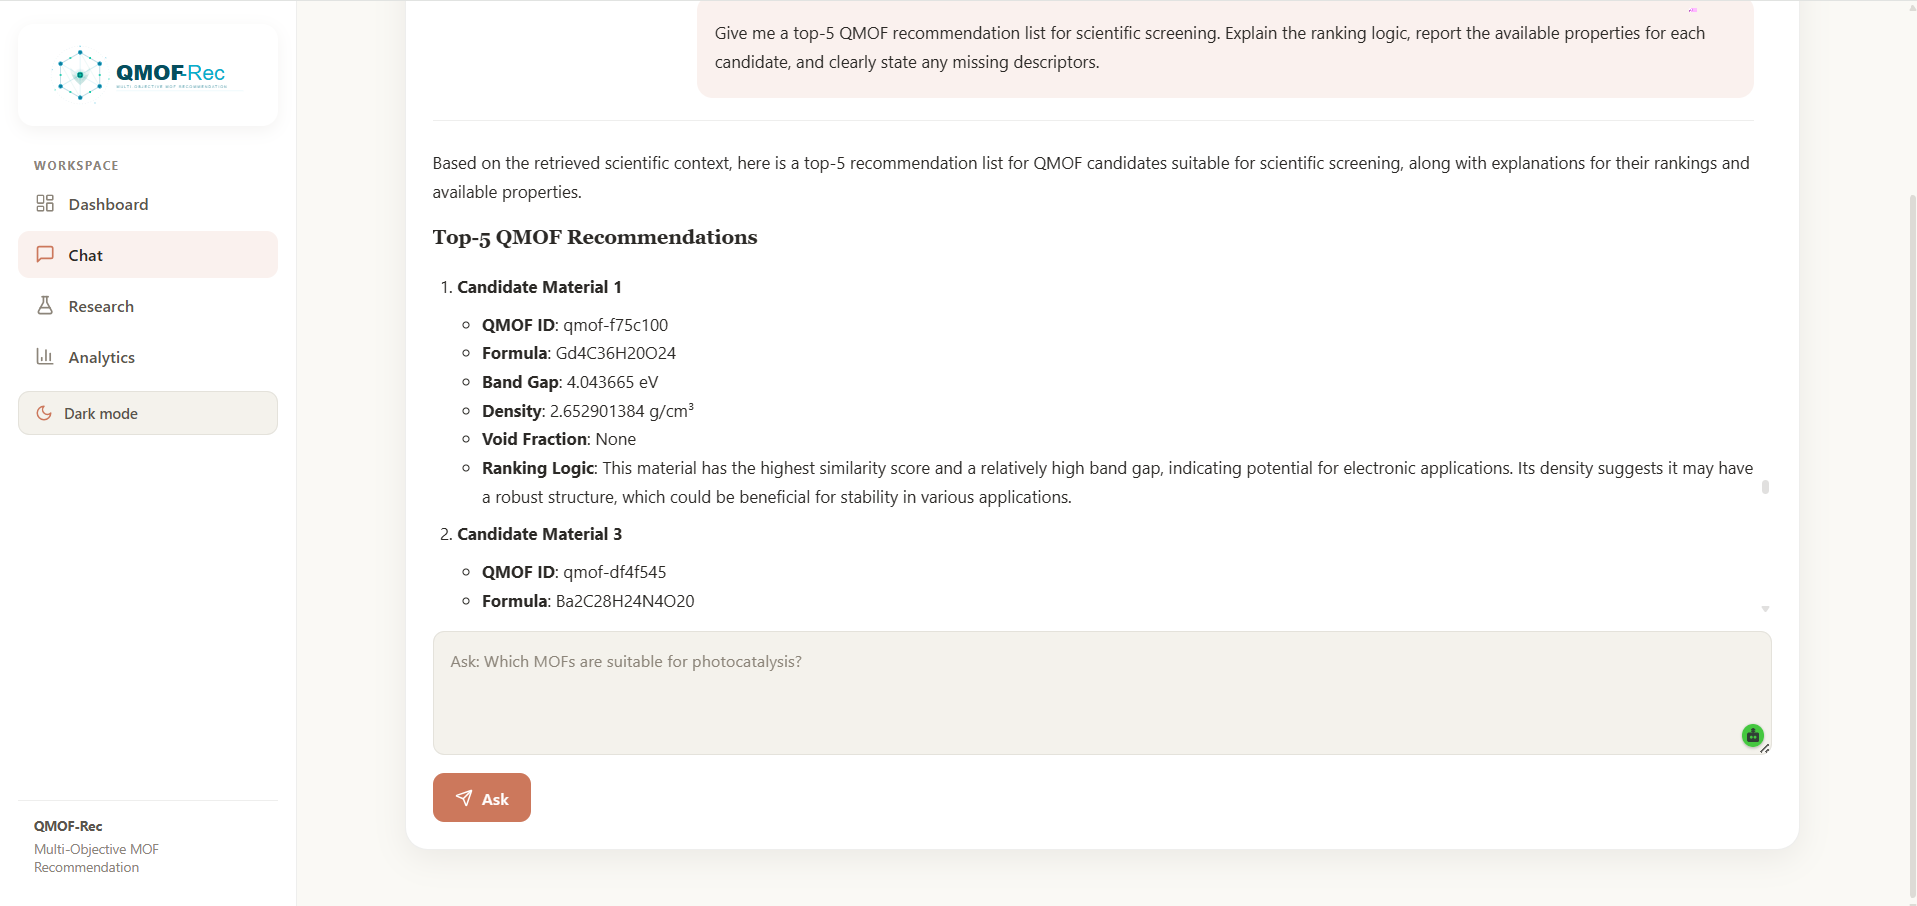
\includegraphics[width=\linewidth]{figures/Scenarion_5a-RankingLogic.png}
  \caption{Ranking-logic scenario. The assistant provides a structured recommendation list with explicit ranking rationale and missing-descriptor reporting.}
\end{figure}

\section*{Interface Example: Candidate Diversity}

\begin{figure}[H]
  \centering
  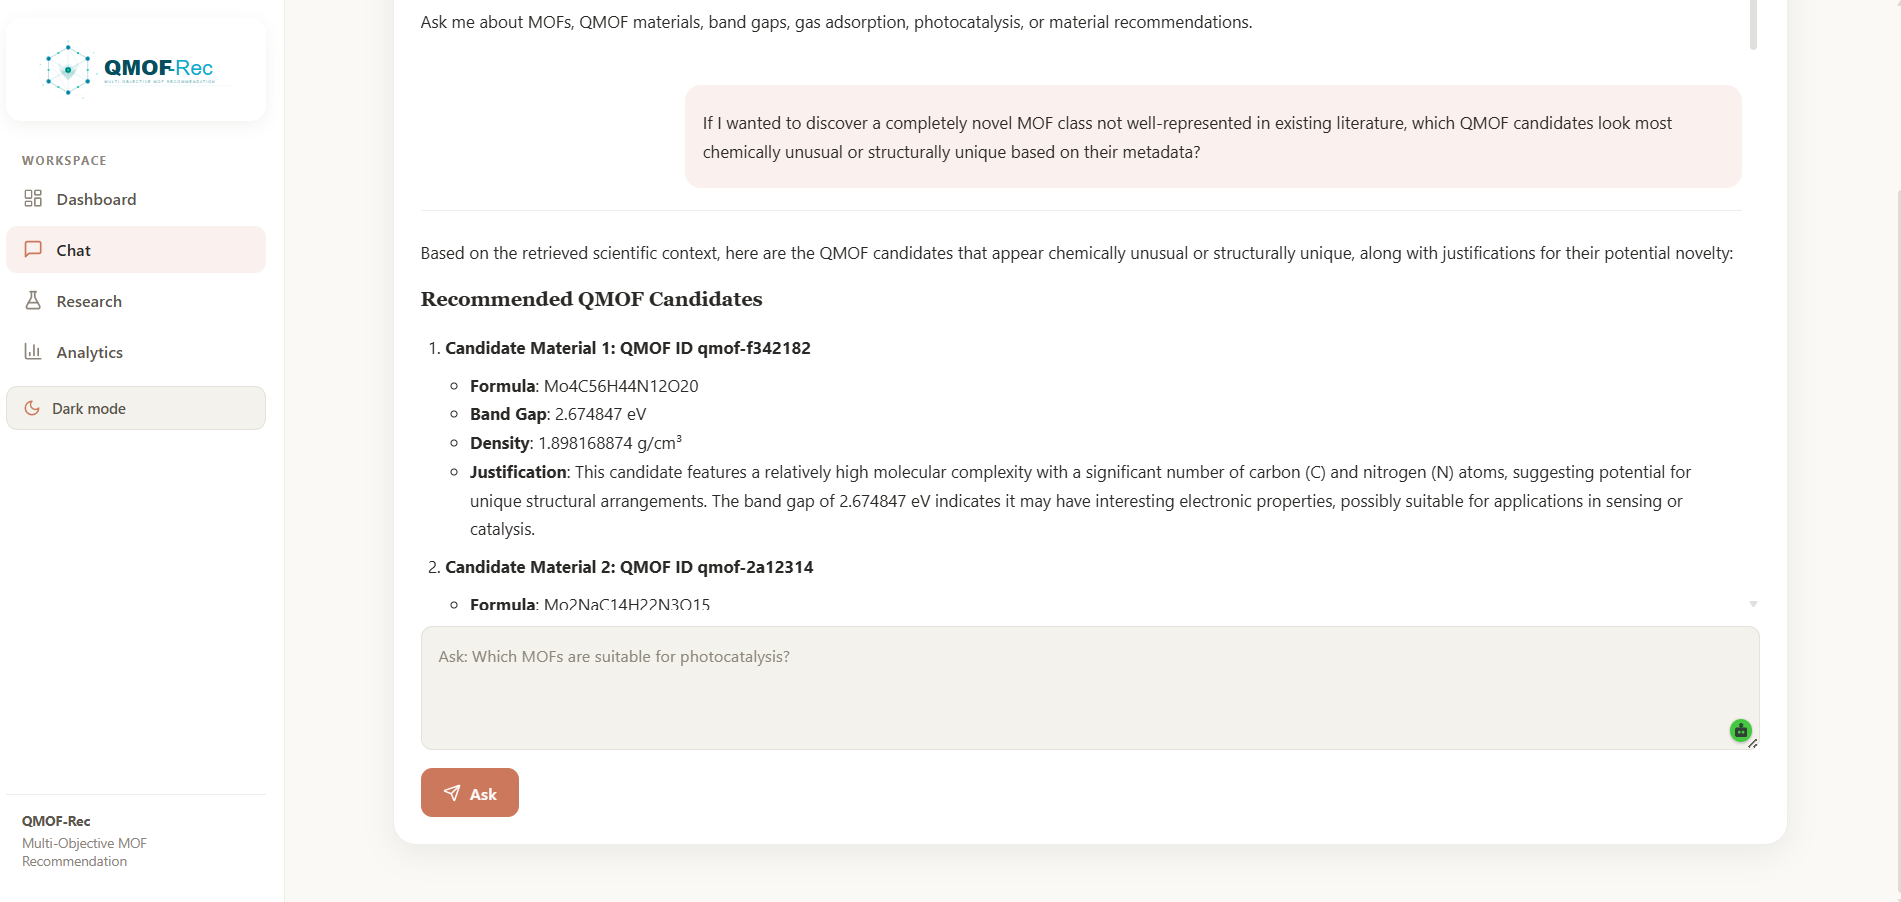
\includegraphics[width=\linewidth]{figures/Scenarion-Chemcallynovel.png}
  \caption{Candidate-diversity interface scenario. The response is grounded in available metadata and should not be interpreted as experimental, adsorption, porosity, or structure-level validation.}
\end{figure}

\end{document}
